\documentclass[a4paper,12pt]{article} 

%%%%%%%%%%%%%%%%%%%%%%%%%%%%%%%% CONSTANTES %%%%%%%%%%%%%%%%%%%%%%%%%%%%%%%%%%%
\newcommand{\numero}{0}                                    %Numéro de la série -1

\usepackage[french]{babel}
\usepackage[utf8]{inputenc}
\usepackage{answers}

\usepackage{hyperref}
\usepackage{multicol}

\usepackage[table,xcdraw]{xcolor}
\usepackage{listings}
\definecolor{ForestGreen}{RGB}{34,139,34}


\usepackage{enumitem}

\AtBeginDocument{\def\labelitemi{$\bullet$}}


\newcommand{\py}{\lstinline{Python} }


\definecolor{backcolour}{rgb}{0.95,0.95,0.92}

\lstset{%
	language         = Python,
	backgroundcolor  = \color{backcolour},
	basicstyle       = \ttfamily, % \upshape\ttfamily,
	keywordstyle     = \bfseries\color{blue}, %\bfseries,
	stringstyle      = \color{magenta},
	commentstyle     = \color{ForestGreen},
	alsoletter = > ,
	morekeywords = {>>>,as,assert,False,None, nonlocal,True, with,yield , <<, >>, :},
	showstringspaces = false,
	numbers=left,
	stepnumber=1,
	literate={à}{{\`{a}}}1 {é}{{\'e}}1 {è}{{\`{e}}}1 {ê}{{\^{e}}}1 {Ê}{{\^{E}}}1 {î}{{\^i}}1 {ô}{{\^{o}}}1 {ç}{{\c{c}}}1 {Ç}{{\c{C}}}1
}

\newcommand{\itemb}[1]{\item \textbf{#1}}

\usepackage{fancyhdr}  %package pour en-tetes et pied de pages
\usepackage{sectsty} % Permet de faire des modifications de police dans diverses sections des "headings" (cf. modif presentation de la page)
\pagestyle{fancy}       %Style pour en-tetes et pieds de pages
\fancyhead[CO,CE]{\sc Série 1\hspace{0.5mm}}
\fancyhead[RO,LE]{Collège Sismondi}  % LaTeX/TEX define \strut to be an invisible box of width zero that extends just enough above and below the baseline. Cela permet d'augementer légèrement la taille en bas de la box de manière à ce qu'elle soit collée à la ligne.
\fancyhead[LO,RE]{\small\ \textsl{1\textsuperscript{ère} année - DO Informatique}}
\fancyfoot[RO,LE]{2021 - 2022}
\fancyfoot[LO,RE]{\small }
\fancyfoot[CO,CE]{\thepage}

\fancyhfoffset[l]{1.2cm} % le "l" en paramètre permet d'indiquer qu'on ne veut modifier que la marge à gauche.
\renewcommand{\headrule}{{%
		\hrule \headwidth \headrulewidth \vskip-\headrulewidth}}
\renewcommand\footrulewidth{\headrulewidth}
\renewcommand{\footrule}{{%
		\vskip-\footruleskip\vskip-\footrulewidth
		\hrule \headwidth \footrulewidth\vskip\footruleskip}}

\usepackage{tikz}
%-------------------------------------------------------------------------------
%---- Eclairage : en encadré sur fond jaune avec symbôle "ampoule" à gauche ----
%-------------------------------------------------------------------------------
\definecolor{coleclairage}{RGB}{255 , 221 , 156}
\definecolor{contoureclairage}{RGB}{255 , 192 , 0}
\newenvironment{eclairage}
{
	\begin{center}%
		\begin{tikzpicture}%
			\node[rectangle, draw=contoureclairage, top color=coleclairage!50, bottom color=coleclairage!140, rounded corners=5pt, inner xsep=5pt, inner ysep=6pt, outer ysep=10pt]\bgroup                     
			\begin{minipage}{0.98\linewidth}
				\begin{minipage}{0.08\linewidth}\centerline{
\includegraphics[scale=1]{Symbole_eclairage.png}}\end{minipage}
				\begin{minipage}{0.89\linewidth}\itshape\footnotesize
				}
				{                		
				\end{minipage}
			\end{minipage}\egroup;%
		\end{tikzpicture}%
	\end{center}%
}

%-------------------------------------------------------------------------------
%---- apprendre : en encadré sur fond jaune avec symbôle "ampoule" à gauche ----
%-------------------------------------------------------------------------------
\definecolor{colapprendre}{RGB}{50,205,50}
\definecolor{contourapprendre}{RGB}{34,139,34}
\newenvironment{apprendre}
{
	\begin{center}%
		\begin{tikzpicture}%
			\node[rectangle, draw=contourapprendre, top color=colapprendre!10, bottom color=colapprendre!50, rounded corners=5pt, inner xsep=5pt, inner ysep=6pt, outer ysep=10pt]\bgroup                     
			\begin{minipage}{0.98\linewidth}
				\begin{minipage}{0.08\linewidth}\centerline{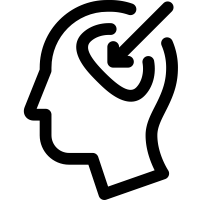
\includegraphics[width=30px]{Symbole_learn.png}}\end{minipage}
				\begin{minipage}{0.89\linewidth}\itshape\footnotesize
				}
				{                		
				\end{minipage}
			\end{minipage}\egroup;%
		\end{tikzpicture}%
	\end{center}%
}

\definecolor{colimportant}{RGB}{247 , 189 , 164}
\definecolor{contourimportant}{RGB}{237 , 125 , 49}
\newenvironment{important}
{
	\begin{center}%
		\begin{tikzpicture}%
			\node[rectangle, draw=contourimportant, top color=colimportant!50, bottom color=colimportant!140, rounded corners=5pt, inner xsep=5pt, inner ysep=6pt, outer ysep=10pt]\bgroup                     
			\begin{minipage}{0.08\linewidth}\centerline{
\includegraphics[scale=0.8]{Symbole_attention.png}}\end{minipage}
			\begin{minipage}{0.89\linewidth}
			}
			{                		
			\end{minipage}\egroup;
		\end{tikzpicture}%
	\end{center}%
}

%-----------------------------------------------------------------
%---- Modification présentation de la page: marges de la page ----
%-----------------------------------------------------------------
%\addtolength{\hoffset}{-1in}              % 1
%\addtolength{\voffset}{-1in}              % 2
\addtolength{\oddsidemargin}{-0.1 in} % 3
\addtolength{\evensidemargin}{-1in} % 3
\addtolength{\topmargin}{-1in}       % 4
\addtolength{\headheight}{6pt}       % 5
%\addtolength{\headsep}{-0.2cm}           % 6
\setlength{\textheight}{26cm}    % 7
\setlength{\textwidth}{16.5cm}      % 8
\addtolength{\marginparsep}{0pt}      % 9
\setlength{\marginparwidth}{0pt}   % 10
\addtolength{\footskip}{-1mm}           %11

\setlength{\parindent}{0em}% pas d'indentation


% Customiser le nom des sections
\usepackage{titlesec}
\titleformat{\section}[hang]{\Large \bfseries}{Série \thesection:\ }{0pt}{}

\renewcommand{\familydefault}{\sfdefault} % pour avoir des polices san serif

\newtheorem{Exc}{Exercice}
\Newassociation{correction}{Soln}{mycor}
\renewcommand{\Solnlabel}[1]{\bfseries Ex #1 }
\def\exo#1{%
	\futurelet\testchar\MaybeOptArgmyexoo}
\def\MaybeOptArgmyexoo{
	\ifx[\testchar \let\next\OptArgmyexoo
	\else \let\next\NoOptArgmyexoo \fi \next}
\def\OptArgmyexoo[#1]{%
	\begin{Exc}[#1]\normalfont}
	\def\NoOptArgmyexoo{%
		\begin{Exc}\normalfont}
		\newcommand{\finexo}{\end{Exc} \vspace{3mm}}
	\newcommand{\flag}[1]{}
	\newcommand{\entete}[1]

\newcommand{\getexocompteur}{{\the\numexpr \arabic{Exc}  \relax}}	
	
\newcommand{\eexo}{\vspace{5mm}} % espace pour séparer les exercices


\begin{document}
%		\title{\vspace{-3cm}Série 1}
%		\date{\vspace{-2cm}}
%		\maketitle

\fancyhead[CO,CE]{\sc Série \arabic{section} \hspace{0.5mm}}
\setcounter{section}{\numero}

\section{Introduction à la programmation}				
\Opensolutionfile{mycor}[cor_01]



\exo{}[L'interpréteur Python]  ~\\ 
\begin{enumerate}
	\item Ouvrir l'éditeur Thonny sur le PC (Kubuntu, MacOS, Windows).
	\item Utilisez Python en mode interactif. Ce mode permet de rapidement tester une commande. Écrivez, dans la console, une à une les lignes suivantes et assurez vous de comprendre le résultat. Pour chaque ligne compléter avec le résultat obtenu :
	\begin{lstlisting}[numbers=none]
>>> 15+3
		
>>> 2 - 17 
		
>>> 8 + 3 * 4 
		
>>> print((8+3)*4)
		
>>> 20 / 3
		
>>> type(5)
		
>>> "Le papa noel dit " + 3*"HO!"
		
>>> print("C'est bizarre.")
		
	\end{lstlisting}
	\item Créez un script nommé  "exercice\_\thesection.\getexocompteur.py" qui contient le code suivant
	\begin{lstlisting}[numbers=none]
15+3
2 - 17 
8 + 3 * 4 
print((8+3)*4)
20 / 3
"Le papa noel dit " + 3*"HO!"
print("C'est bizarre.")	
	\end{lstlisting}
	puis exécutez le programme, que constatez-vous?
	
\end{enumerate}
\finexo


\begin{eclairage}
	Lorsque \py interprète un programme à part d'un fichier alors il n'affiche pas le résultat de l'évaluation de chaque expression. Pour afficher une donnée il faut utiliser la commande \lstinline{print}.
\end{eclairage}

\exo{}[Premier programme]  ~\\ 
\begin{enumerate}
	\item Créer un nouveau fichier dans l'éditeur appelé "exercice\_\thesection.\getexocompteur.py" qui contient le code suivant:
	\lstinputlisting[label={premierprg},numbers=none ]
	{codes/premier_prog_python.py}
	\item Exécuter le programme dans Thonny instruction après instruction en mode débogueur (voir le tutoriel) afin de comprendre que fait le programme.
\end{enumerate}
\begin{center}
	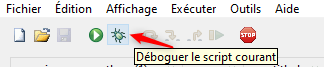
\includegraphics{Thonny-debug.png}
\end{center}
\finexo
%%%%%%%%%%%%%%%%%%%%%%%%%%%%%%%%             EXERCICE              %%%%%%%%%%%%%%%%%%%%%%%%%%%%
\exo{}[première modification]  ~\\ 
	\begin{enumerate}
		\item Créer un nouveau fichier dans l'éditeur appelé "exercice\_\thesection.\getexocompteur.py" qui contient le code suivant
		\lstinputlisting[numbers=none]{codes/verif_age.py}
		\item Enregistrer sur votre Google drive (classroom) le fichier "exercice\_\thesection.\getexocompteur.py" dans un dossier dédié aux exercices du chapitre "série\thesection"?
		\item Quel est le but de ce programme?
		\item Inspirez-vous de l'exemple ci-dessus pour écrire un programme qui vérifie l'âge d'un client d'un bar à New York afin de savoir s'il a le droit de consommer de l'alcool.\\ \textit{Rappel: au État-Unis, la consommation d'alcool est interdite en dessous de 21 ans.}
	\end{enumerate}
	\begin{correction}
		~\\ \vspace{-5pt}
		\lstinputlisting[numbers=none]{codes/corr_exo_verif_age.py}
	\end{correction}
\finexo

\begin{apprendre}
	Pour communiquer avec l'utilisateur le langage \py propose deux fonctions de bases:
	\begin{itemize}
		\item \lstinline{print} qui permet d'afficher une donné ou un message.\\
		Exemple: \lstinline{print("C'est bizarre.")}
		\item \lstinline{input} qui interrompt le programme et attend que l'utilisateur entre une donnée et la valide avec \textit{Enter}.\\
		Exemple: \lstinline{input("Quel est votre age ? ")}
	\end{itemize}
\end{apprendre}

\cleardoublepage

% Solution		
		\newpage
		\setcounter{page}{1}
		\setcounter{section}{\numero}
		\Closesolutionfile{mycor}
		\titleformat{\section}[hang]{\Large \bfseries}{Corrigé Série \thesection:\ }{0pt}{}
		

		\fancyhead[CO,CE]{\sc Corrigé Série \arabic{section} \hspace{0.5mm}}
		\section{}
		\Readsolutionfile{mycor}
	\end{document}